% Plantilla simple para tareas de la Licenciatura en Física
% Fer Flores - Universidad de Guadalajara - Noviembre 2023

%%%%%%%%%%%%%%%%%%%%%%%%%%%%%%%%%%%%%%%%%%-PREÁMBULO-%%%%%%%%%%%%%%%%%%%%%%%%%%%%%%%%%%%%%%%%%%

% Paqueterías

\documentclass{assignment}
\usepackage[pdftex]{graphicx} % FIGURAS
\usepackage{xcolor}
\definecolor{LightGray}{gray}{0.95}
\usepackage{fancyvrb, minted} % CÓDIGO
\usepackage[letterpaper, margin = 2.5cm]{geometry} % TAMAÑO DE PÁGINA Y MÁRGENES
\usepackage[T1]{fontenc} % Importante para acentos automáticos y símbolos de escritura
\usepackage[spanish, mexico]{babel} % Importante para Español
\usepackage{amsmath, amsfonts, amssymb} % Ecuaciones, caracteres y símbolos especiales
\usepackage{hyperref, url}  % Links y Hyperlinks en el documento
\usepackage{fancyhdr}

%-----------------------------------------ETIQUETAS--------------------------------------------

\student{Elad Siman Tov}                             % NOMBRE
\semester{Winter 2024}                                % SEMESTRE (202X A/B)
\date{\today}                                   % Fecha (Modifica a DD/MM/AAAA)

\courselabel{Neural Networks}          % CLAVE Y MATERIA
\exercisesheet{Homework 1}{Neural Networks}     % NÚMERO Y TÍTULO DE LA TAREA

\school{Mechanical Engineering}          % CARERA (Física, la mejor carrera)
\university{Technion Israel Institute for Technology}         % LA PODEROSÍSIMA

%%%%%%%%%%%%%%%%%%%%%%%%%%%%%%%%%%%%%%%%%%-DOCUMENTO-%%%%%%%%%%%%%%%%%%%%%%%%%%%%%%%%%%%%%%%%%%%%

\begin{document}

%-----------------------------------------------------------------------------------------------
\begin{problem}

\section{Reading}

\noindent I hereby declare that I have read chapter 1 from the Course textbook - \href{https://udlbook.github.io/udlbook/}{Understanding Deep Learning}. 

\section{Theory}
\begin{enumerate}
    \item Option C:
    Machine Learning is a branch of artificial intelligence that enables systems to learn from data and make predictions or decision.
    \item Option C:
     The main goal of supervised learning is minimizing the error between predicted and actual outputs
     \item Option C:
     An example of unsupervised learning is Customer segmentation.
     \item Option B:
     The purpose of a validation set in machine learning is to measure the model’s performance on unseen data and tune hyper-parameters.
     \item Option D:
     Over-fitting in machine learning is when the model memorizes the training data and performs poorly on unseen data.
     \item Option C:
     The purpose of feature scaling in machine learning is to standardize or normalize the numerical features to a common scale.
     \item Option B:
     The appropriate evaluation metrics for a binary classification problem is the F1-Score.
     \item Option A:
     The role of a loss function in a machine learning model is to measure the distance between predicted and actual values.
     \item Option D:
     The purpose of cross-validation in machine learning is to prevent over-fitting by using multiple validation sets.
     \item Option A:
     The machine learning algorithms used for both classification and regression are Random Forests, KNN and SVM (Under some modifications)
\end{enumerate}

\section{Prerequisites}

\noindent 


\noindent Recuerda los distintos tipos de ecuaciones que puedes agregar a tu documento:

\begin{itemize}
    \item Para una ecuación sencilla utilizamos el método \texttt{equation}, que encerramos con \texttt{boxed}:
    \begin{equation}\label{eq:Sencilla}
        \boxed{             % Así la encerramos para destacarla
        e^{\pi i} + 1 = 0
        }
    \end{equation}

    \item Podemos referenciar la ecuación anterior con el método \texttt{ref}: (Ec. \ref{eq:Sencilla}). Para una ecuación larga utilizamos el método \texttt{multiline}. Además, podemos agregar un asterisco (*) si no queremos numerarla:
    \begin{multline*}
        p(x) = 3x^6 + 14x^5y + 590x^4y^2 + 19x^3y^3 - 12x^2y^4 + 12xy^5 + 2y^6 - a^3b^3\\ 
            - 12x^2y^4 - 12xy^5 + 2y^6 - a^3b^3 + 3x^6 + 14x^5y - 590x^4y^2 + 19x^3y^3
    \end{multline*}

    \item Para dividir la ecuación larga en dos líneas o más (para por ejemplo mostrar un proceso de simplificación o de operaciones) utilizamos el comando \texttt{split}:
    \begin{equation} \label{eq1}
        \begin{split}
            A & = \frac{\pi r^2}{2} \\
             & = \frac{1}{2} \pi r^2
        \end{split}
    \end{equation}

    \item Para mostrar un \textit{sistema} de ecuaciones, utilizamos el ambiente \texttt{align}: 
    \begin{align*} 
        2x - 5y &=  8 \\ 
        3x + 9y &=  -12
    \end{align*}
    Que también podemos aplicar a sistemas más complejos:
    \begin{align*}
        x&=y           &  w &=z              &  a&=b+c\\
        2x&=-y         &  3w&=\frac{1}{2}z   &  a&=b\\
        -4 + 5x&=2+y   &  w+2&=-1+w          &  ab&=cb
    \end{align*}    

    \item Para \textit{agrupar} ecuaciones consecutivamente sin alineamiento, utilizamos \texttt{gather}:
    \begin{gather*} 
        2x - 5y =  8 \\ 
        3x^2 + 9y =  3a + c
    \end{gather*}
\end{itemize}

\noindent Muchas veces en nuestras tareas incorporamos imágenes como a la que hacemos referencia aquí (Figura \ref{fig:yo_en_la_vida}):
\begin{figure}[ht] % Especificamos ubicacion (h = aquí mero)
    \centering
    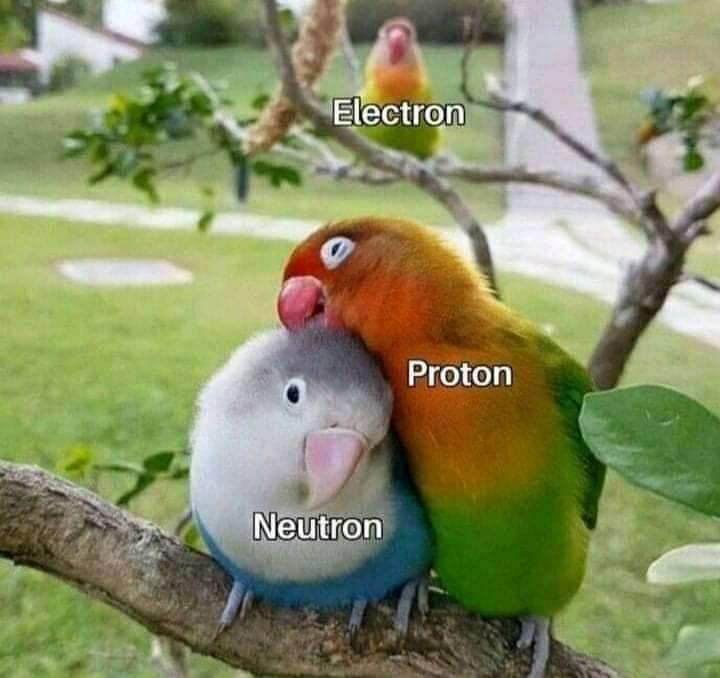
\includegraphics[width=0.5\textwidth]{Figuras/Cotorros.jpg} % Ancho especificado
    \caption{Esquema de las relaciones entre los componentes del núcleo atómico}
    \label{fig:yo_en_la_vida}
\end{figure}

\noindent Finalmente, recuerda utilizar el método \texttt{minted} para escribir el código que incluyas en tu tarea, y \texttt{verbatim} para el \textit{pseudo}-código\footnote{Muchas veces es mejor incluír \textit{ambos} para darte a entender con tu profesor}:

\begin{minted}[frame=lines, linenos, bgcolor=LightGray]{python}
    def funcion(argumento1, argumento2):
        """
        Explico que hace la funcón
        """
        if condicion == True:
            alumno = graduado
        else:
            alumno = baja
\end{minted}

\end{problem}
%---------------------------------------------------------------------------------------------
% \begin{problem}

% \section{Segundo Problema}

% \noindent
    
% \end{problem}
%---------------------------------------------------------------------------------------------



%--------------------------------------BIBLIOGRAFIA-------------------------------------------

\newpage

\nocite{*} % Agrega las referencias aunque no las hayas citado directamente

\bibliographystyle{unsrt}    % ESTILO DE BIBLIOGRAFÍA (Recomendados: abbrv, ieeetr, apalike, unsrt)
\bibliography{refs}     % REFERENCIAS EN ARCHIVO SEPARADO


\end{document}
